\documentclass{sig-alternate}
\usepackage{float}
\usepackage{listings}
\usepackage{color}
\restylefloat{table}

\title{CSCI-620 Data Management with the IMDb Dataset}
\subtitle{[Developing tools to interact with the IMDb dataset]}
\numberofauthors{4}
\author
{
	\alignauthor
	Aishwarya Rao
	\email{ar2711@rit.edu}
	\alignauthor
	Apurav Khare
	\email{ak2816@rit.edu}
	\and
	\alignauthor
	Martin Qian
	\email{jq3513@rit.edu}
	\alignauthor
	Prateek Kalasannavar
	\email{pk6685@rit.edu}
}

\definecolor{dkgreen}{rgb}{0,0.6,0}
\definecolor{gray}{rgb}{0.5,0.5,0.5}
\definecolor{mauve}{rgb}{0.58,0,0.82}

\lstset{frame=tb,
  language=SQL,
  aboveskip=3mm,
  belowskip=3mm,
  showstringspaces=false,
  columns=flexible,
  basicstyle={\small\ttfamily},
  numbers=none,
  numberstyle=\tiny\color{gray},
  keywordstyle=\color{blue},
  commentstyle=\color{dkgreen},
  stringstyle=\color{mauve},
  breaklines=true,
  breakatwhitespace=true,
  tabsize=3
}

\begin{document}
	\maketitle
	\begin{abstract}
		This project aims to explore a dataset by understanding it, modeling it to a normalized relational schema so that it can be stored and retrieved from a relational database management system. The project also focuses on developing an interface that allows fast and easy access to the dataset by abstracting complex query scenarios, like search by specific parameters within and across tables, and aggregate queries.
	\end{abstract}
	
	\section{Project Status}
	As established in Phase 0 and Phase 1, the deliverable of Phase 2 in Data Management includes three things. One, a document specifying different query scenarios on the IMDb dataset, their equivalent queries and sample outputs. Two, a script that handles requests from the user interface and maps these requests to the relevant query and responds with appropriate results. Finally, a user interface that allows the user to pick scenarios, specify various filters and view the results in a readable format.
	The following sections cover the technology and methodology used to implement these tasks, query scenarios, and screenshots of the output. 
	\subsection{Technology Used}
	We used a web interface that allows users to interact with our database through a browser. The front end is built with ReactJS and BootStrap. It consists of tabs for every query scenario and allows entry of appropriate filters as seen in \ref{frontend}. On submitting a customized query, the request is handled by a Python script which uses the the user entered values to build a query and sends it to the database. It collects the response and sends it back to ReactJS for the user to view. \newline
	The database is stored using Microsoft SQL Server 2017 and the queries are built accordingly.
	\begin{figure}[ht]
		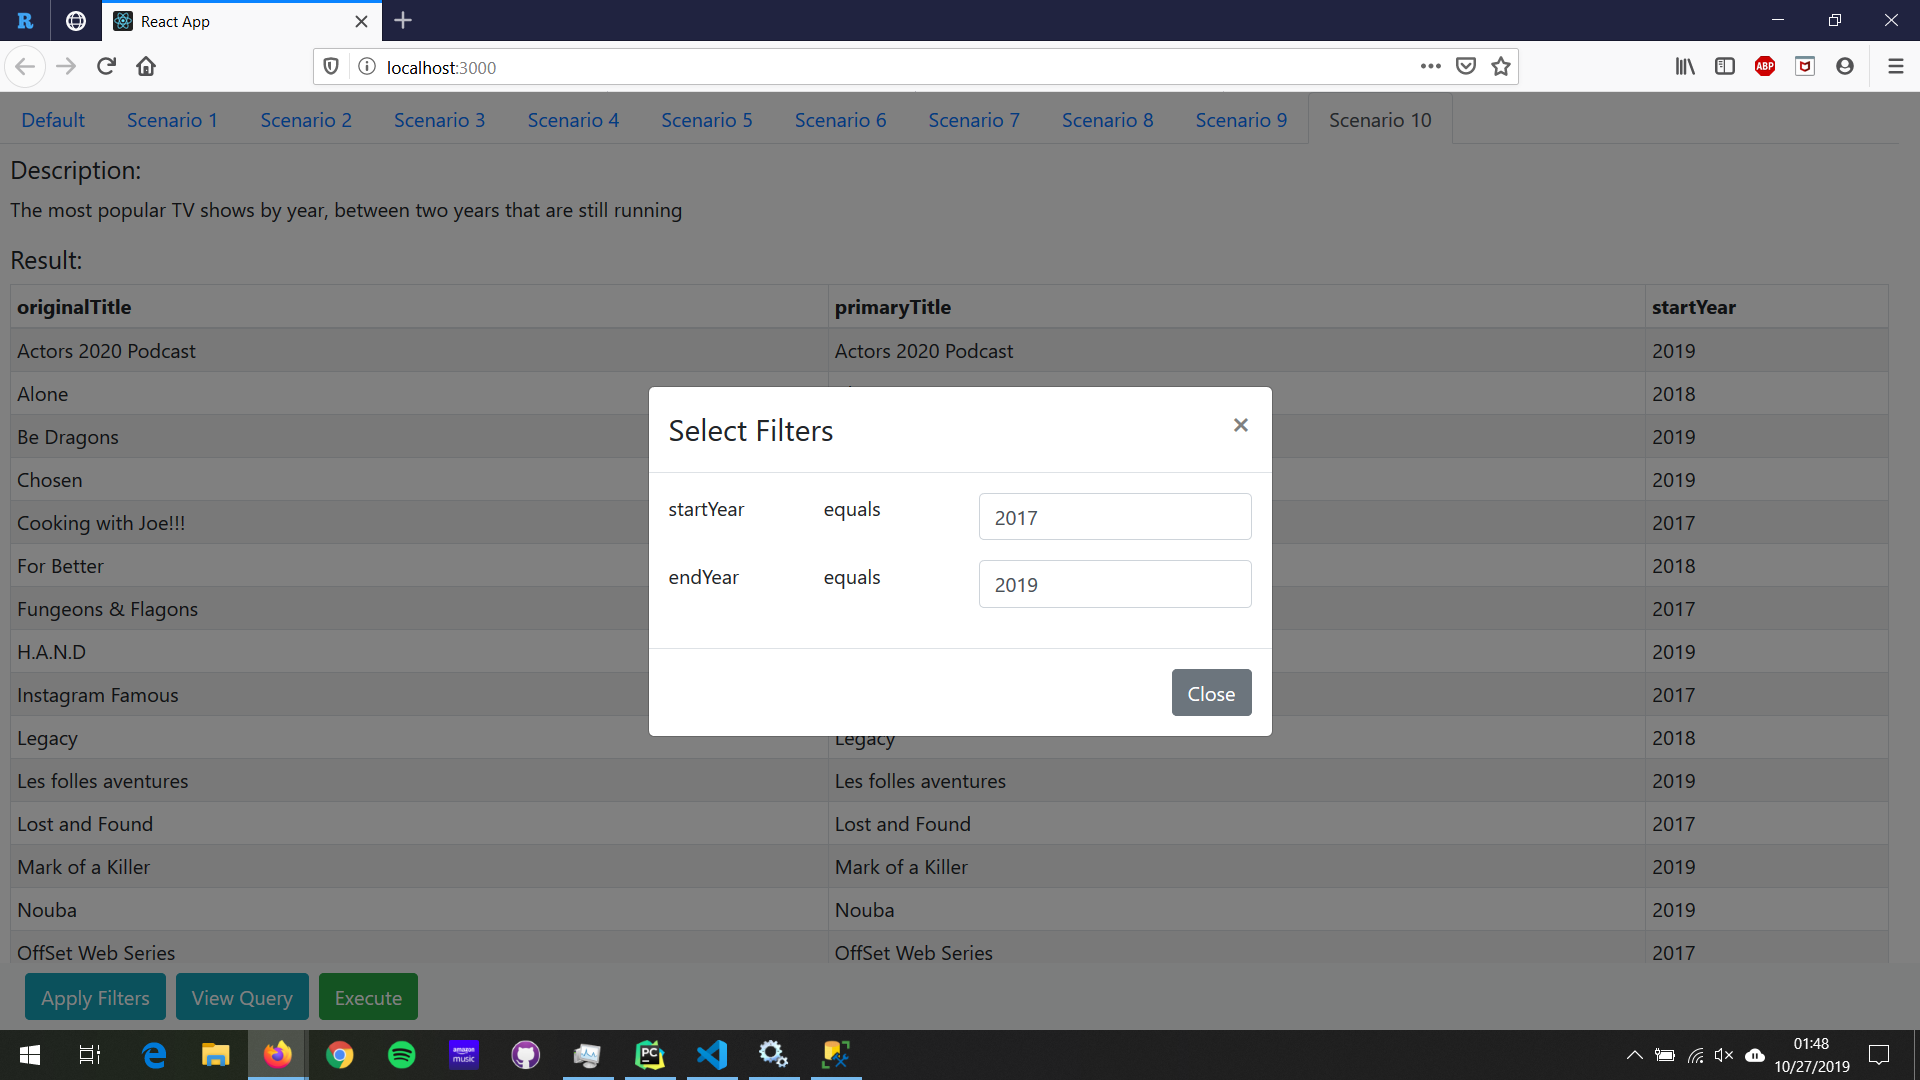
\includegraphics[width=8cm]{Screenshots/Frontend.png}
                \caption{Front-end - Applying applicable filters}
		\label{frontend}
		\centering
	\end{figure}
\subsection{Requirements and running the code}
Our development phases uses the following technologies,
\begin{itemize}
	\item Python 3.6 with Flask
	\item ReactJS 
	\item Microsoft SQL Server 2017
\end{itemize}
Due to memory and storage constraints, the database size was cut down to only those entries after the year 2000. The related tables are adjusted accordingly.
\subsection{Performance considerations}
	SQL Server creates clustered indexes for all columns in the primary key. In addition to that, we added non-clustered indexes on columns that were frequently used for look-up in the tables. These include the year and name columns in the title and name tables, and genre column in the titleGenres table. Indexes are added using the following scripts:
        \begin{lstlisting}
CREATE INDEX IX_title_name on title(originalTitle);
CREATE INDEX IX_title_year on title(startYear);
CREATE INDEX IX_name_name on name(primaryName);
CREATE INDEX IX_name_year on name(deathYear);
CREATE INDEX IX_genre on titleGenres(genre);
        \end{lstlisting}
        Overall, a 10-15\% performance improvement was observed in the queries that filter on the non-text (deathYear and startYear) columns after applying the indexes.
	\subsection{Query Scenarios}
	\begin{enumerate}
		\item List the names of alive actors whose name starts with a given keyword (such as “Phi”)and did not participate in any movie in a given year (such as 2014)\\
                \begin{lstlisting}
SELECT name.primaryName FROM name, movie, principalCast
WHERE name.primaryName = principalCast.primaryName
AND name.birthYear = principalCast.birthYear AND principalCast.category = 'actor'
AND movie.startYear NOT IN (SELECT startYear FROM movie WHERE startYear <> 2017)
AND name.deathYear IS NULL AND principalCast.primaryTitle = movie.primaryTitle
AND principalCast.originalTitle = movie.originalTitle AND principalCast.startYear = movie.startYear
AND name.primaryName LIKE 'phi';
                \end{lstlisting}

         	\begin{figure}[ht]
		    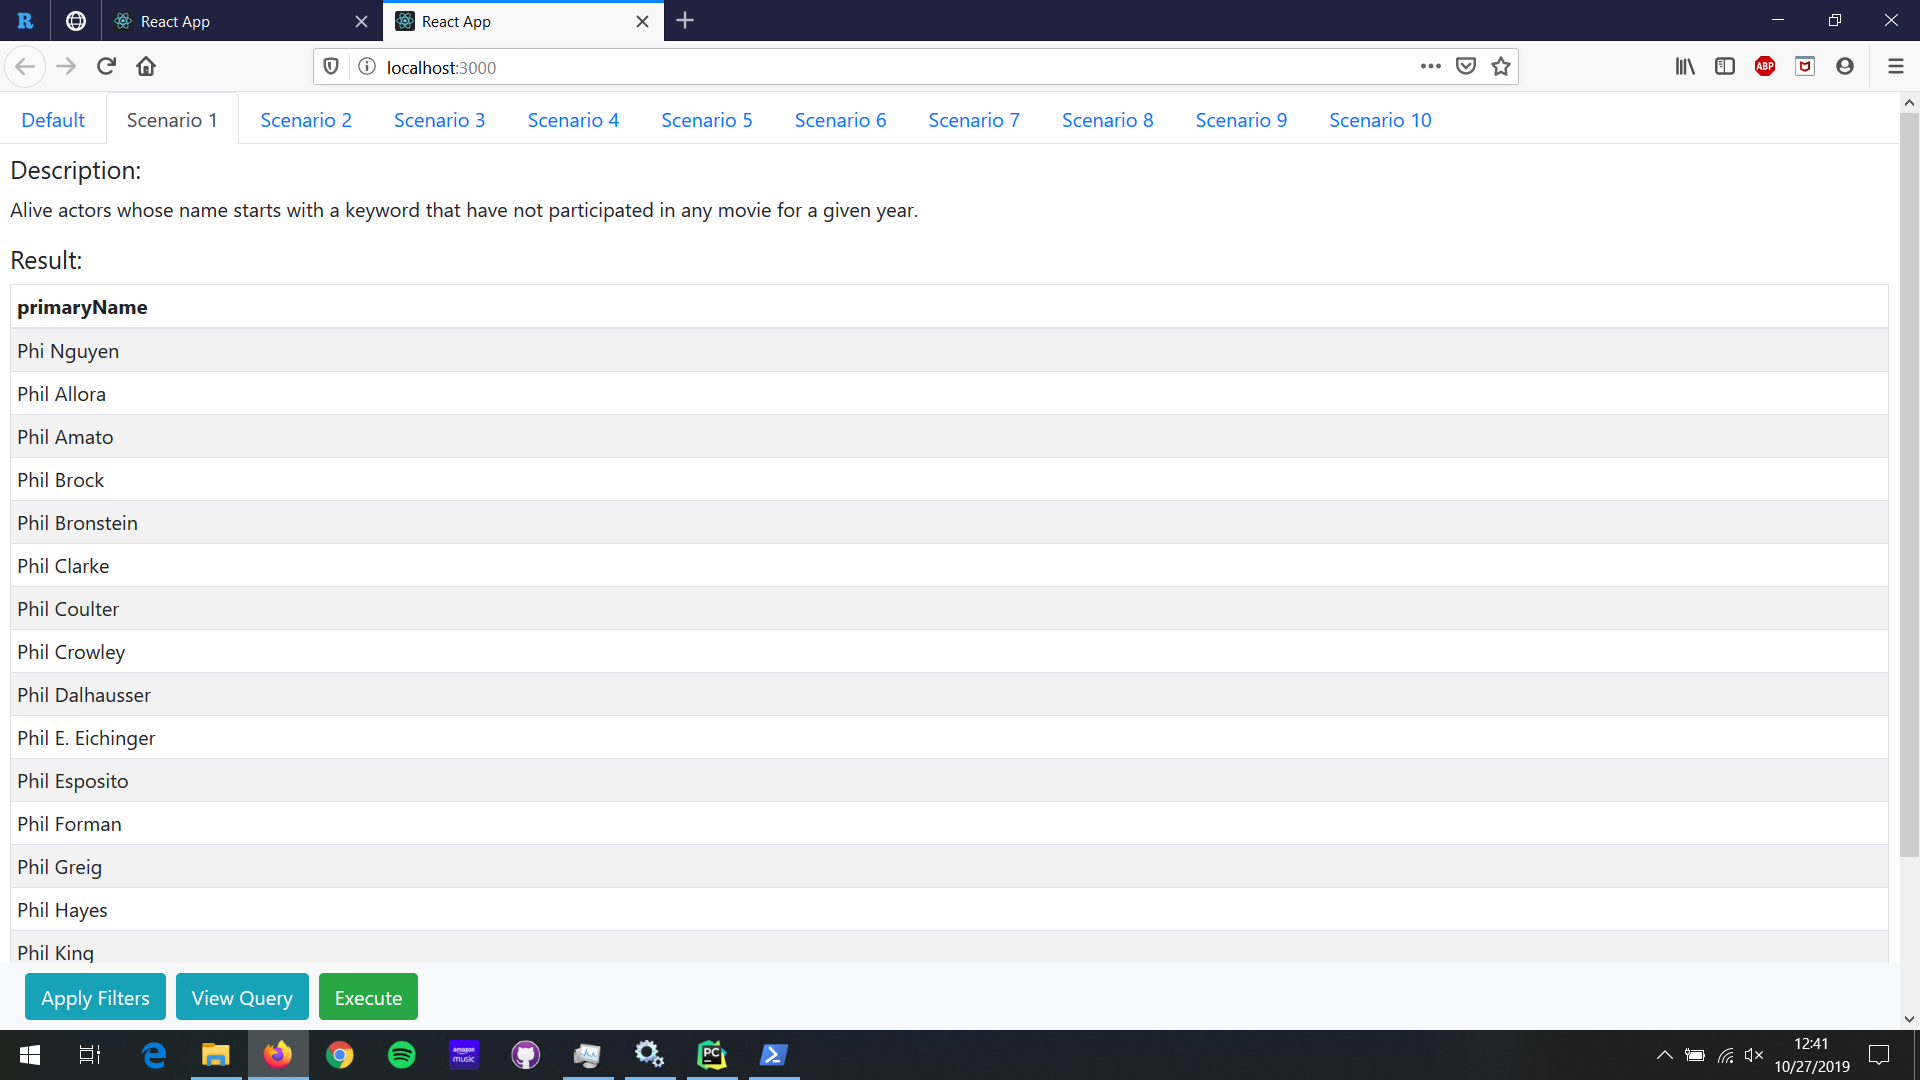
\includegraphics[width=8cm]{Screenshots/Scenario1.png}
		    \label{frontend}
                    \caption{Scenario 1 Result}
		    \centering
	        \end{figure}
		\item List the names of alive producers who have produced more than a given number (such as 50) of talk  shows in a  given  year  (such  as 2017) and  whose  name contains  a  given  keyword  (such  as “Gill”)
                \begin{lstlisting}
SELECT n.primaryName
FROM name n
inner join principalCast pc on pc.primaryName = n.primaryName and pc.birthYear = n.birthYear
inner join titleGenres tg on tg.originalName = pc.originalName and tg.primaryTitle = pc.primaryTitle and tg.startYear = pc.startYear
where n.deathYear is null and tg.genre = 'talk-show' and tg.startYear = 2017 and n.primaryName like 'gill%'
group by n.primaryName
having count(tg.originalTitle) >= 50;
                \end{lstlisting}
         	\begin{figure}[ht]
		    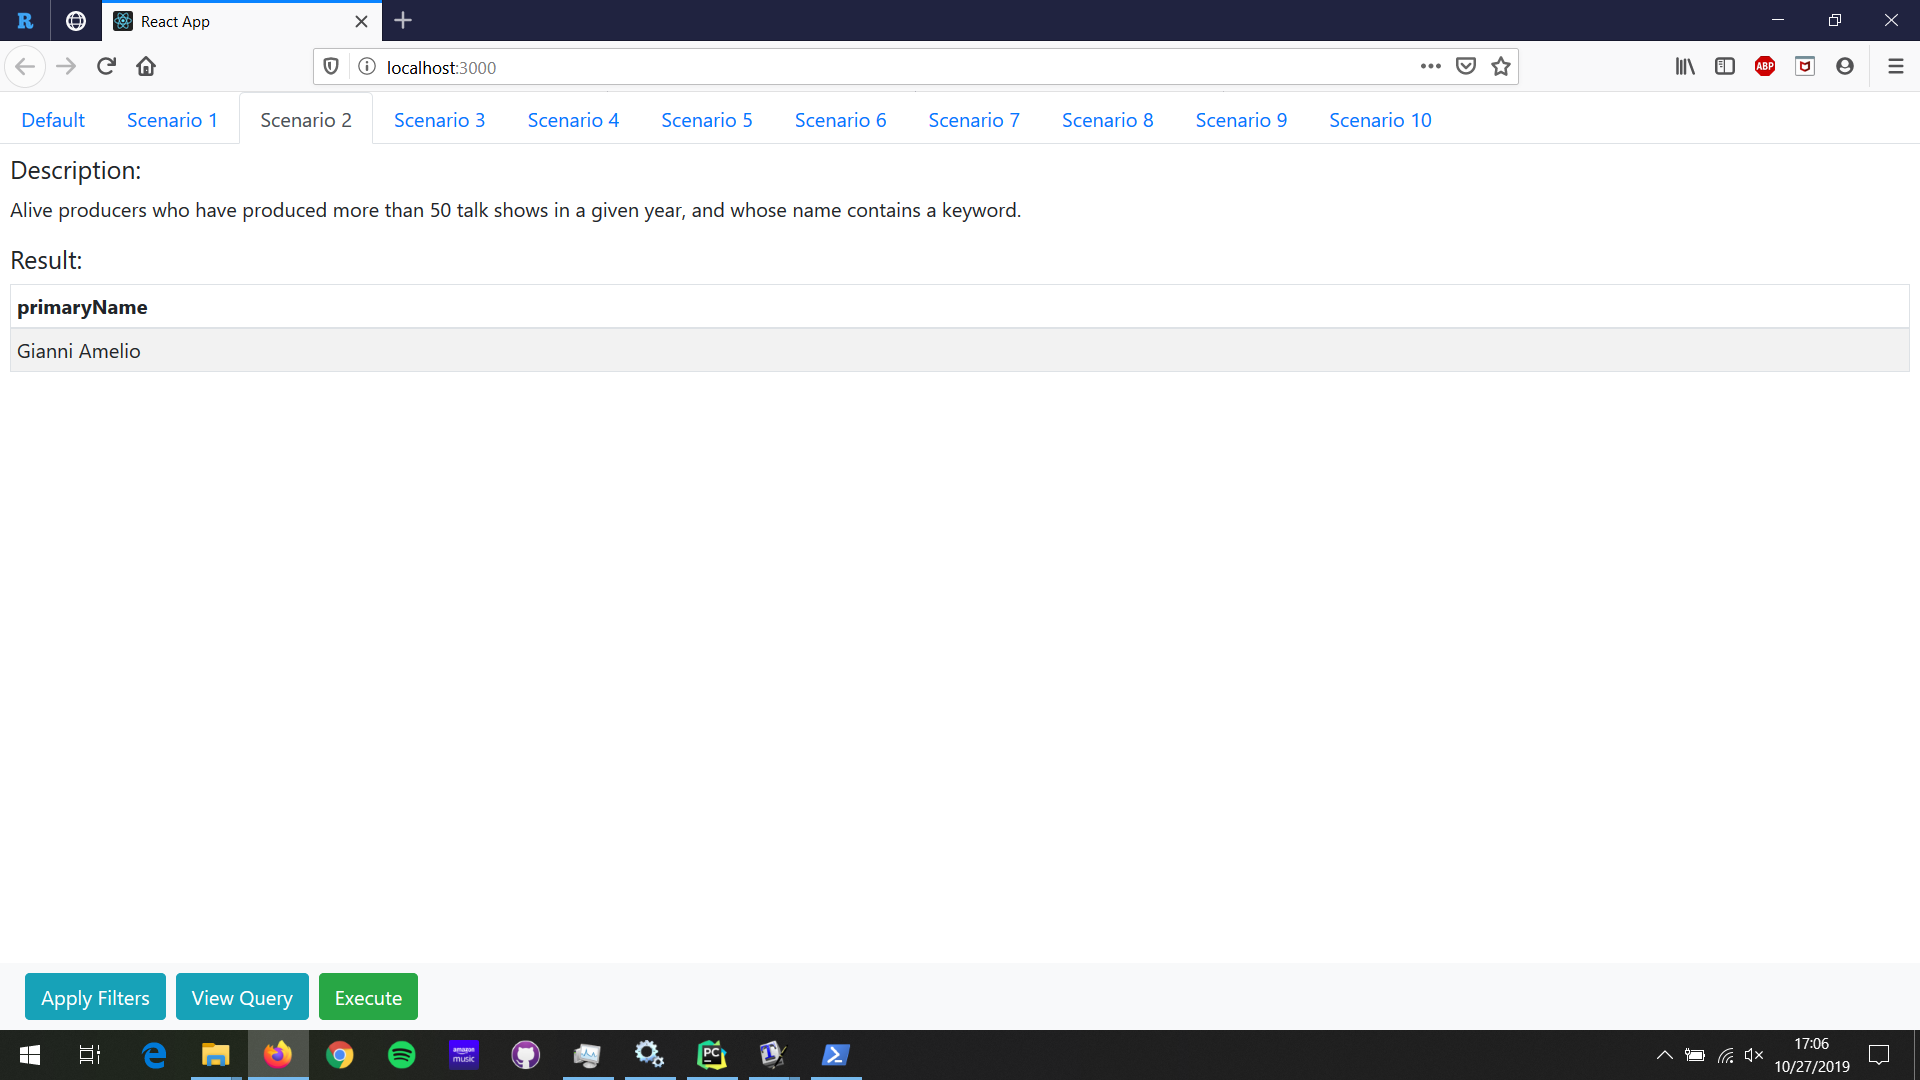
\includegraphics[width=8cm]{Screenshots/Scenario2.png}
		    \label{frontend}
                    \caption{Scenario 2 Result}
		    \centering
	        \end{figure}
		\item List the average runtime for movies whose original title contain a given keyword such as (“star”)and were written by somebody who is still alive
                \begin{lstlisting}
SELECT top 100 avg(runtimeInMinutes) as AverageRunTime FROM movie, title,writers, name
WHERE movie.primaryTitle = title.primaryTitle
AND movie.originalTitle = title.originalTitle AND movie.startYear = title.startYear
AND writers.primaryTitle = title.primaryTitle AND writers.originalTitle = title.originalTitle
AND writers.startYear = title.startYear AND writers.primaryName = name.primaryName
AND writers.birthYear = name.birthYear AND name.deathYear IS NULL
AND movie.originalTitle LIKE '%gill%';
                \end{lstlisting}

         	\begin{figure}[ht]
		    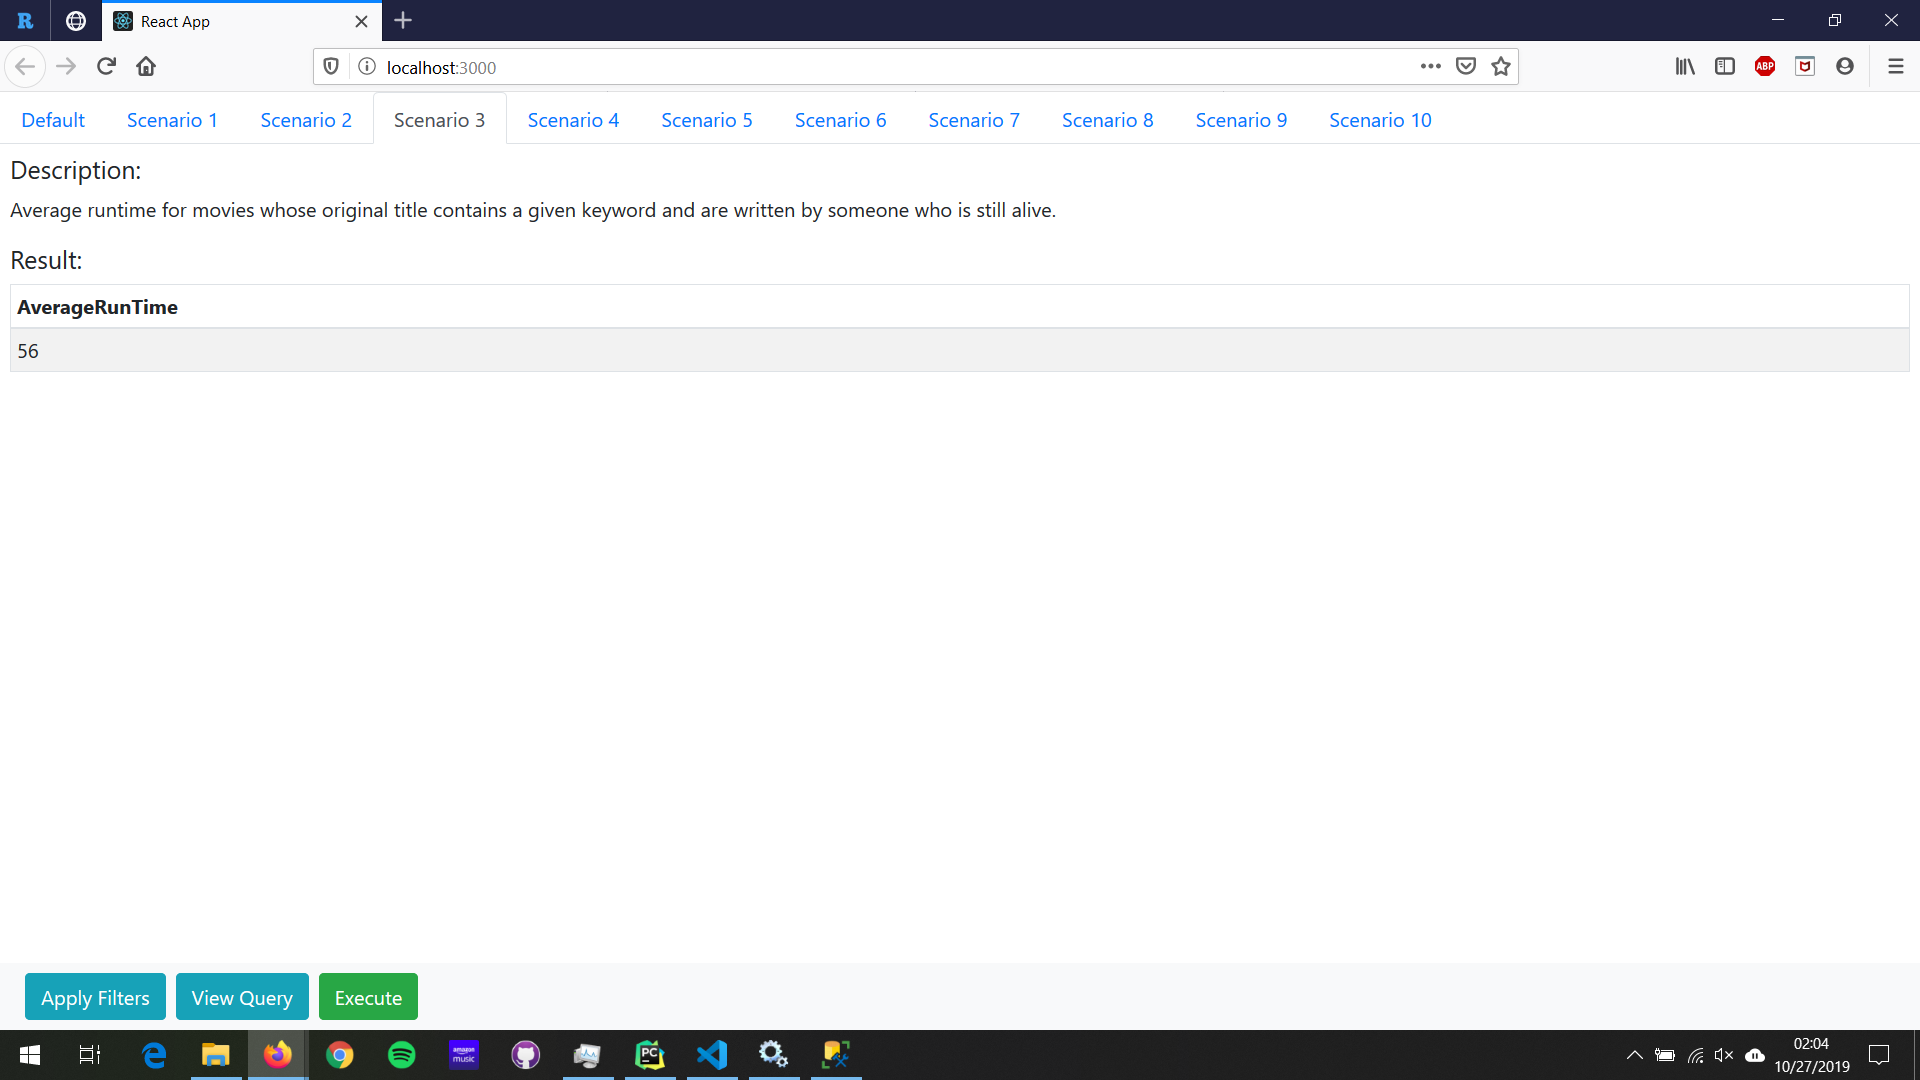
\includegraphics[width=8cm]{Screenshots/Scenario3.png}
		    \label{frontend}
                    \caption{Scenario 3 Result}
		    \centering
	        \end{figure}
		\item List the names of alive producers with the greatest number of long-run movies produced (runtime greater than 120min)
                \begin{lstlisting}
SELECT name.primaryName from name, movie, title, principalCast
WHERE principalCast.primaryName = name.primaryName
AND principalCast.birthYear = name.birthYear
AND principalCast.primaryTitle = title.primaryTitle
AND principalCast.originalTitle = title.originalTitle
AND principalCast.startYear = title.startYear
AND movie.primaryTitle = title.primaryTitle
AND movie.originalTitle = title.originalTitle
AND movie.startYear = title.startYear
AND title.runtimeInMinutes > 120
AND name.deathYear IS NULL
GROUP BY name.primaryName
HAVING count(movie.originalTitle) >=
(Select Max(totalCounts) from
(SELECT COUNT(movie.originalTitle) AS totalcounts FROM name n, movie m, title t, principalCast p
WHERE p.primaryName = n.primaryName
AND p.birthYear = n.birthYear
AND p.primaryTitle = t.primaryTitle
AND p.originalTitle = t.originalTitle
AND p.startYear = t.startYear
AND m.primaryTitle = t.primaryTitle
AND m.originalTitle = t.originalTitle
AND m.startYear = t.startYear
AND t.runtimeInMinutes > 120
AND n.deathYear IS NULL) tc)
                \end{lstlisting}
         	\begin{figure}[ht]
		    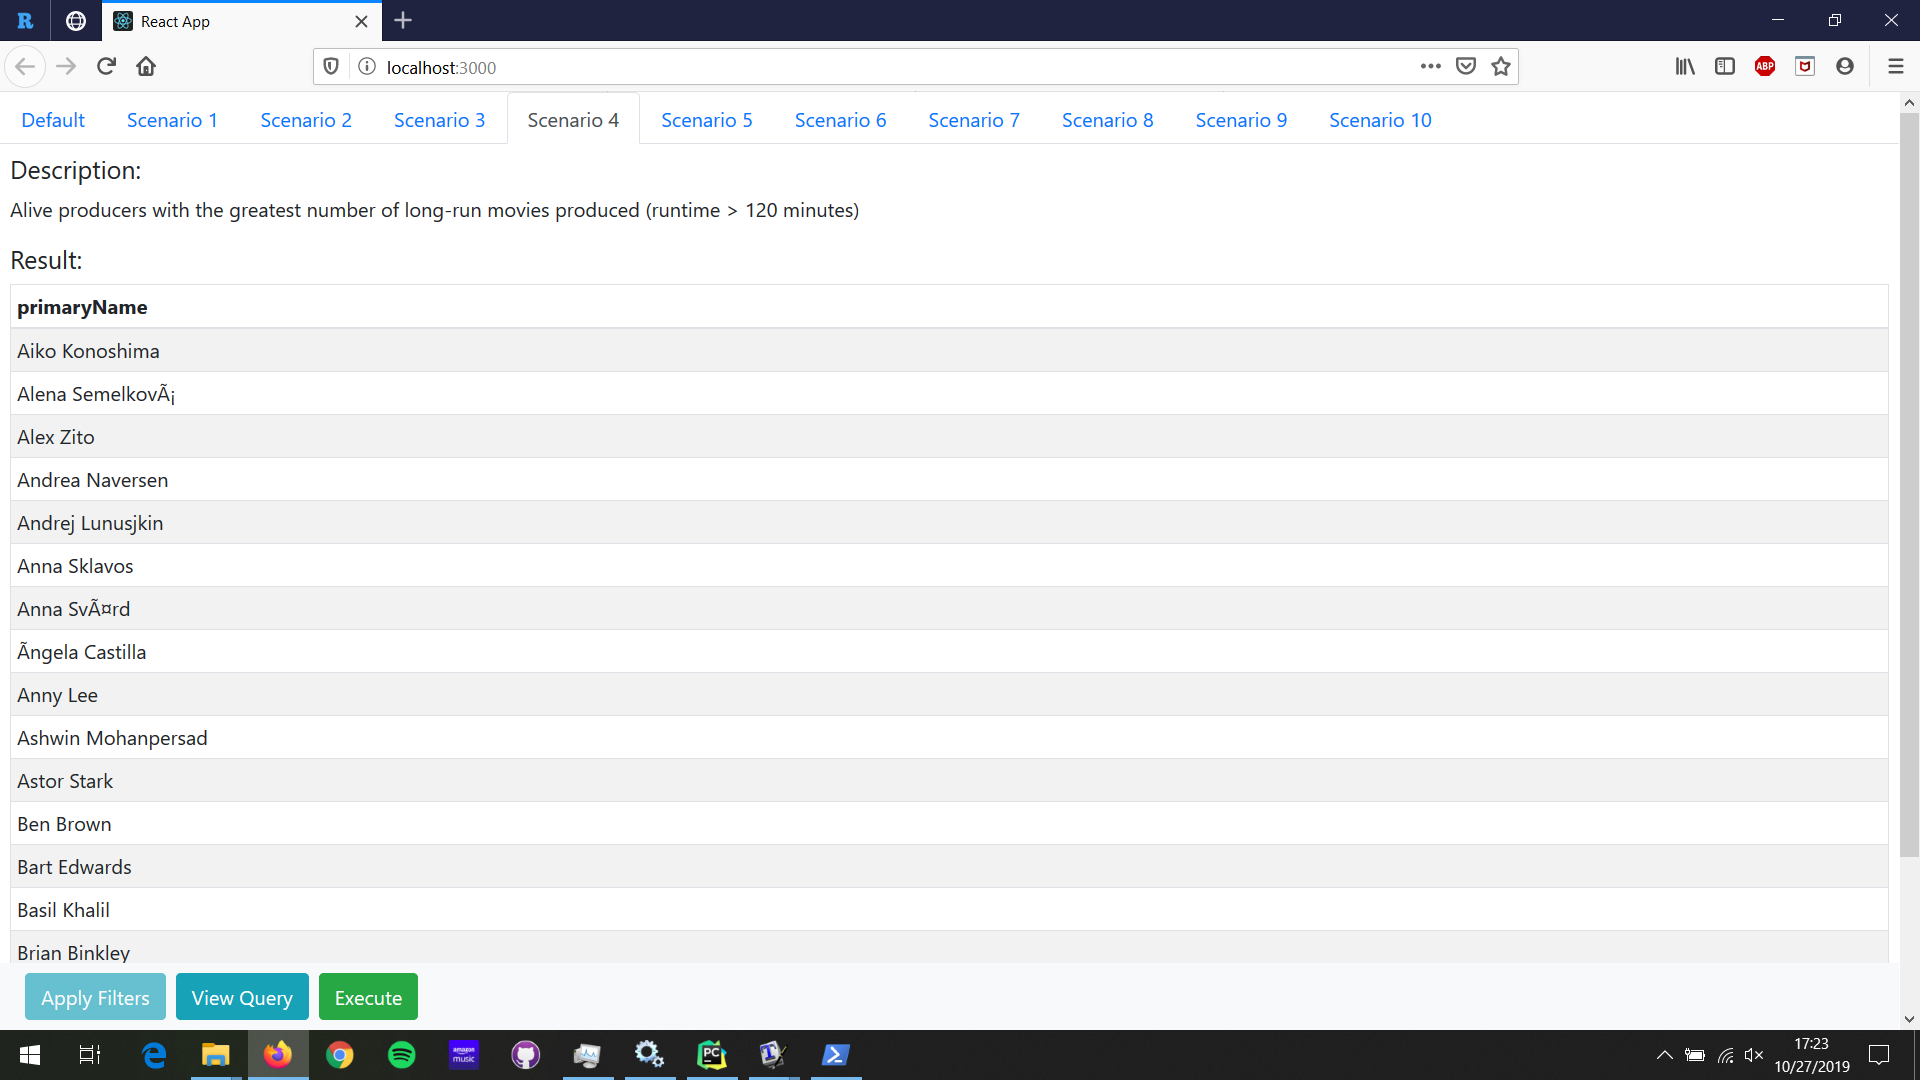
\includegraphics[width=8cm]{Screenshots/Scenario4.png}
		    \label{frontend}
                    \caption{Scenario 4 Result}
		    \centering
	        \end{figure}
		\item List the unique name pairs of actors who have acted together in more than a given number (such as 2)  movies and sort them by average movie rating (of those they acted together).
                \begin{lstlisting}
SELECT Aname.primaryName, Bname.primaryName, AVG(averageRating)
FROM name Aname,name Bname, movie, title, principalCast Apc, principalCast Bpc
WHERE Aname.primaryName = Apc.primaryName 
AND Aname.birthYear = Apc.birthYear 
AND Bname.primaryName = Bpc.primaryName 
AND Bname.birthYear = Bpc.birthYear
AND Aname.birthYear <> Bname.birthYear 
AND Aname.primaryName <> Bname.primaryName
AND movie.originalTitle = title.originalTitle 
AND movie.primaryTitle = title.primaryTitle
AND movie.startYear = title.startYear 
AND Apc.originalTitle = title.originalTitle 
AND Apc.primaryTitle = title.primaryTitle 
AND Apc.startYear = title.startYear 
AND Bpc.originalTitle = title.originalTitle 
AND Bpc.primaryTitle = title.primaryTitle
AND Bpc.startYear = title.startYear 
GROUP BY Aname.primaryName, Bname.primaryName
HAVING COUNT(movie.originalTitle)>=2;
                \end{lstlisting}
         	\begin{figure}[ht]
		    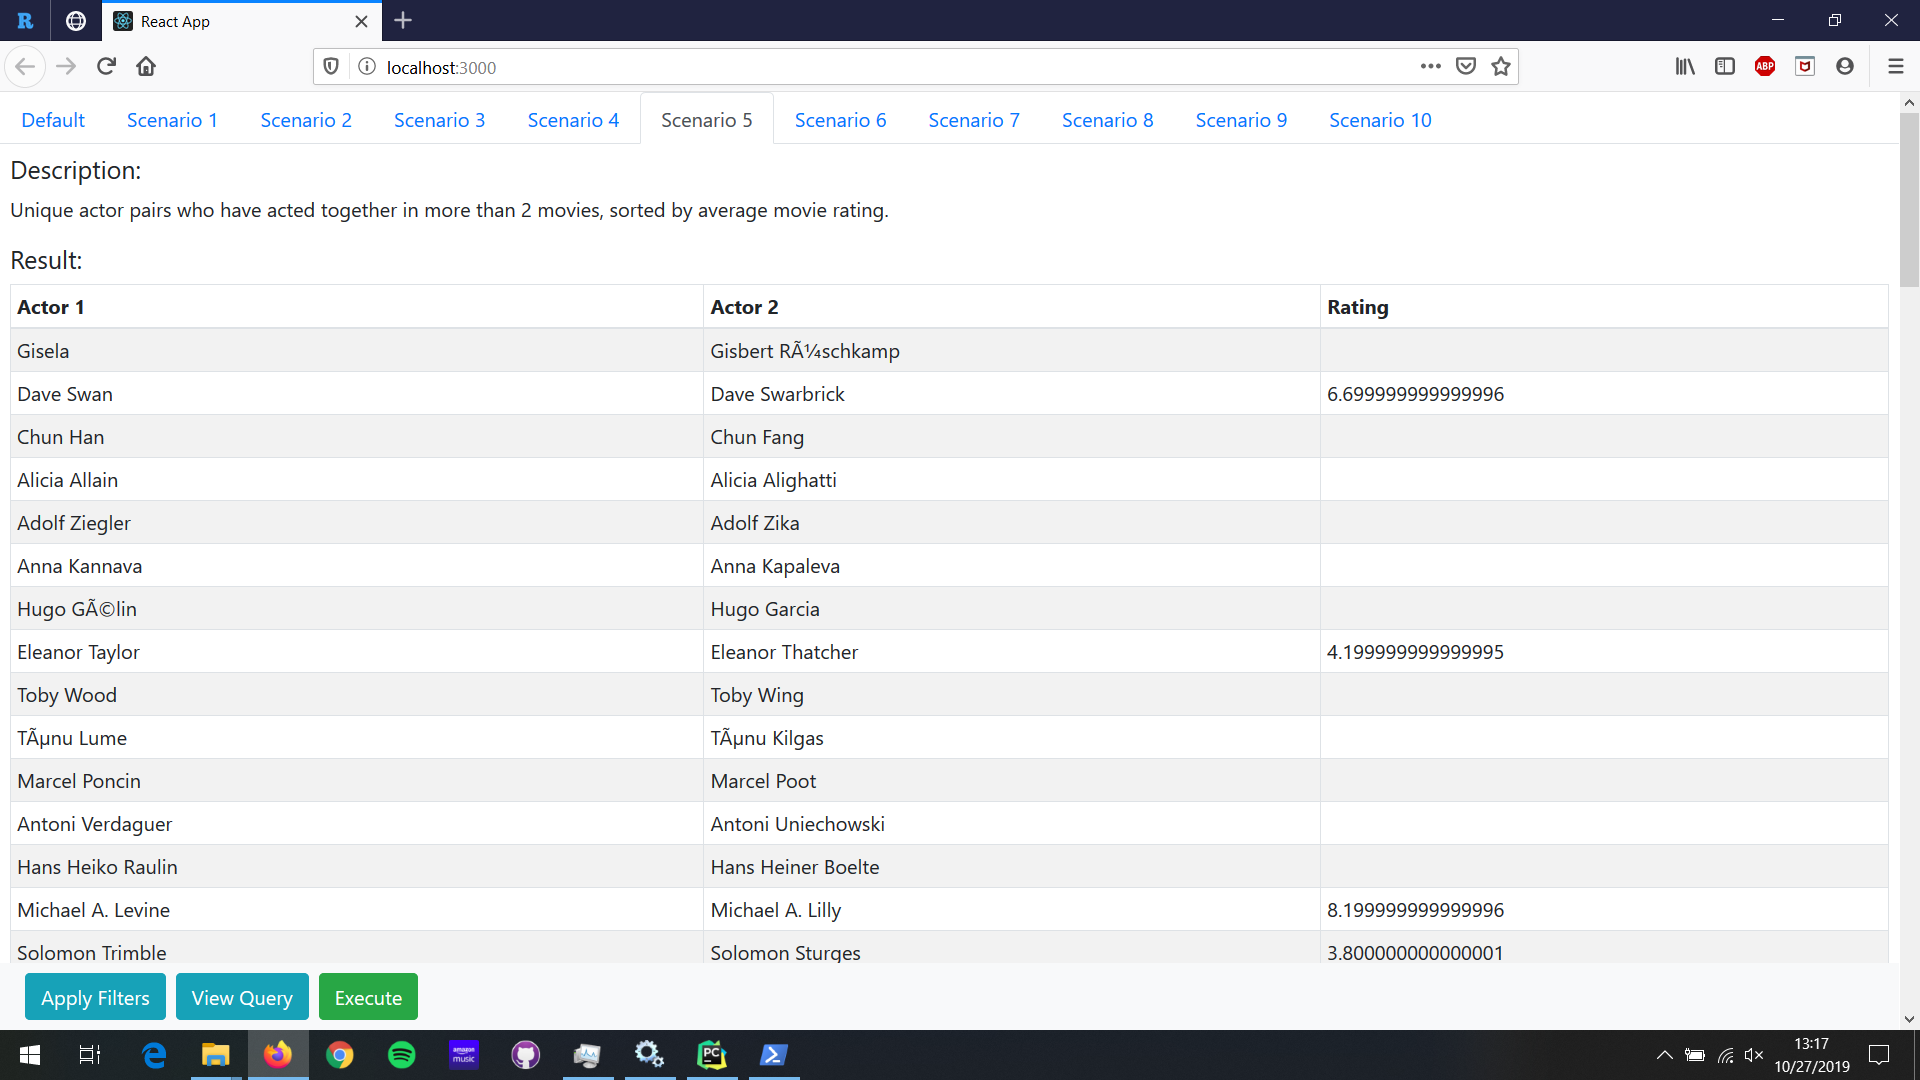
\includegraphics[width=8cm]{Screenshots/Scenario5.png}
		    \label{frontend}
                    \caption{Scenario 5 Result}
		    \centering
	        \end{figure}
		\item List the actors that have worked in x movies (say 10) from one genre (say horror)
                \begin{lstlisting}
SELECT n.primaryName FROM name n
inner join principalCast pc on pc.primaryName = n.primaryName and pc.birthYear = n.birthYear
inner join movie m on m.originalTitle = pc.originalTitle and m.primaryTitle = pc.primaryTitle and m.startYear = pc.startYear
inner join titleGenres tg on tg.originalTitle = m.originalTitle and tg.primaryTitle = m.primaryTitle and tg.startYear = m.startYear
where tg.genre = 'horror' and m.movieType = 'movie' and pc.category = 'actor'
group by n.primaryName, n.birthYear
having COUNT(CONCAT(pc.originalTitle, pc.primaryTitle, pc.startYear)) > 10;
                \end{lstlisting}
         	\begin{figure}[ht]
		    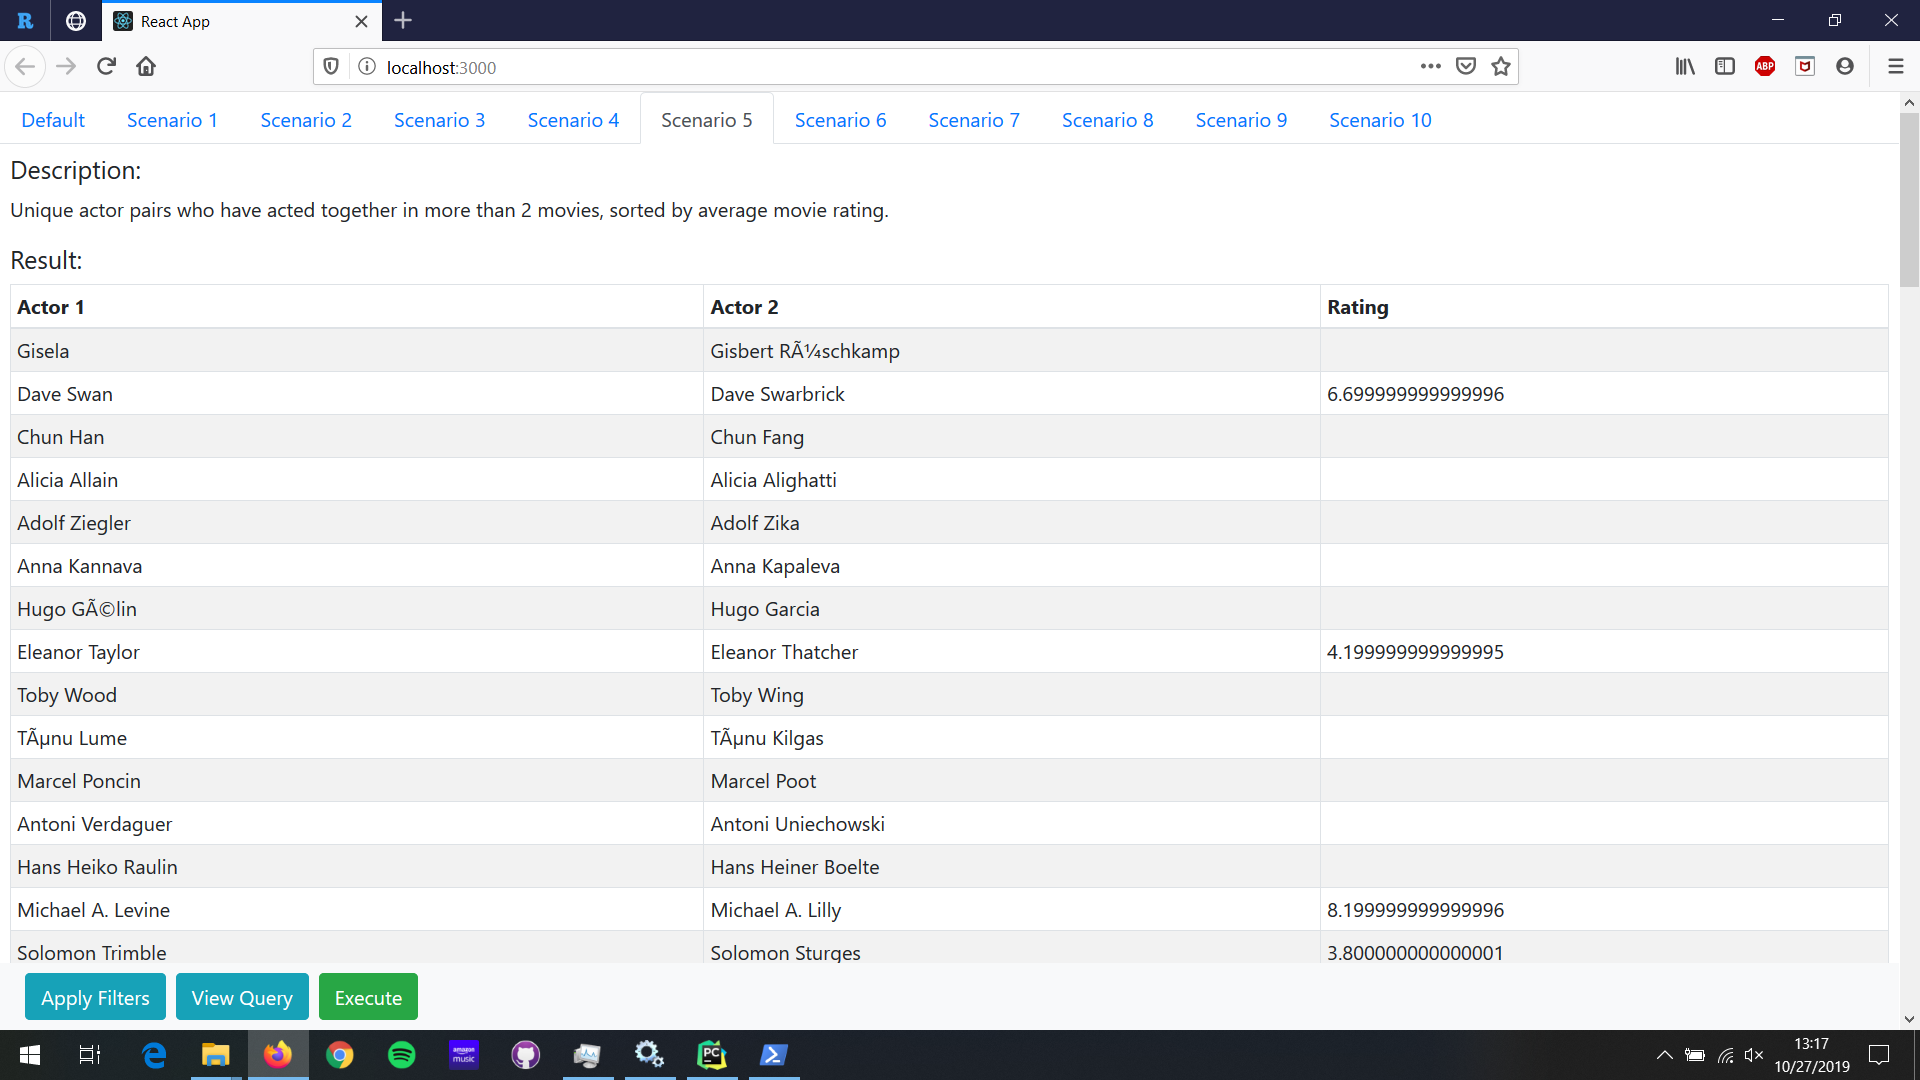
\includegraphics[width=8cm]{Screenshots/Scenario5.png}
		    \label{frontend}
                    \caption{Scenario 6 Result}
		    \centering
	        \end{figure}
		\item Actors and directors that have worked together certain number of times in titles that are not tv shows and the titles that they have worked in together.
                \begin{lstlisting}
select n.primaryName as actor, d.primaryName as director, d.originalTitle, m.movieType
from name n
inner join principalCast pc on pc.primaryName = n.primaryName and pc.birthYear = n.birthYear
inner join directors d on d.originalTitle = pc.originalTitle and d.startYear = pc.startYear
inner join movie m on m.originalTitle = d.originalTitle and m.primaryTitle = d.primaryTitle and m.startYear = d.startYear
where pc.category = 'actor'
group by n.primaryName, n.birthYear, d.primaryName, d.birthYear
having COUNT(CONCAT(d.originalTitle, d.primaryTitle, d.startYear)) > 5;
                \end{lstlisting}
         	\begin{figure}[ht]
		    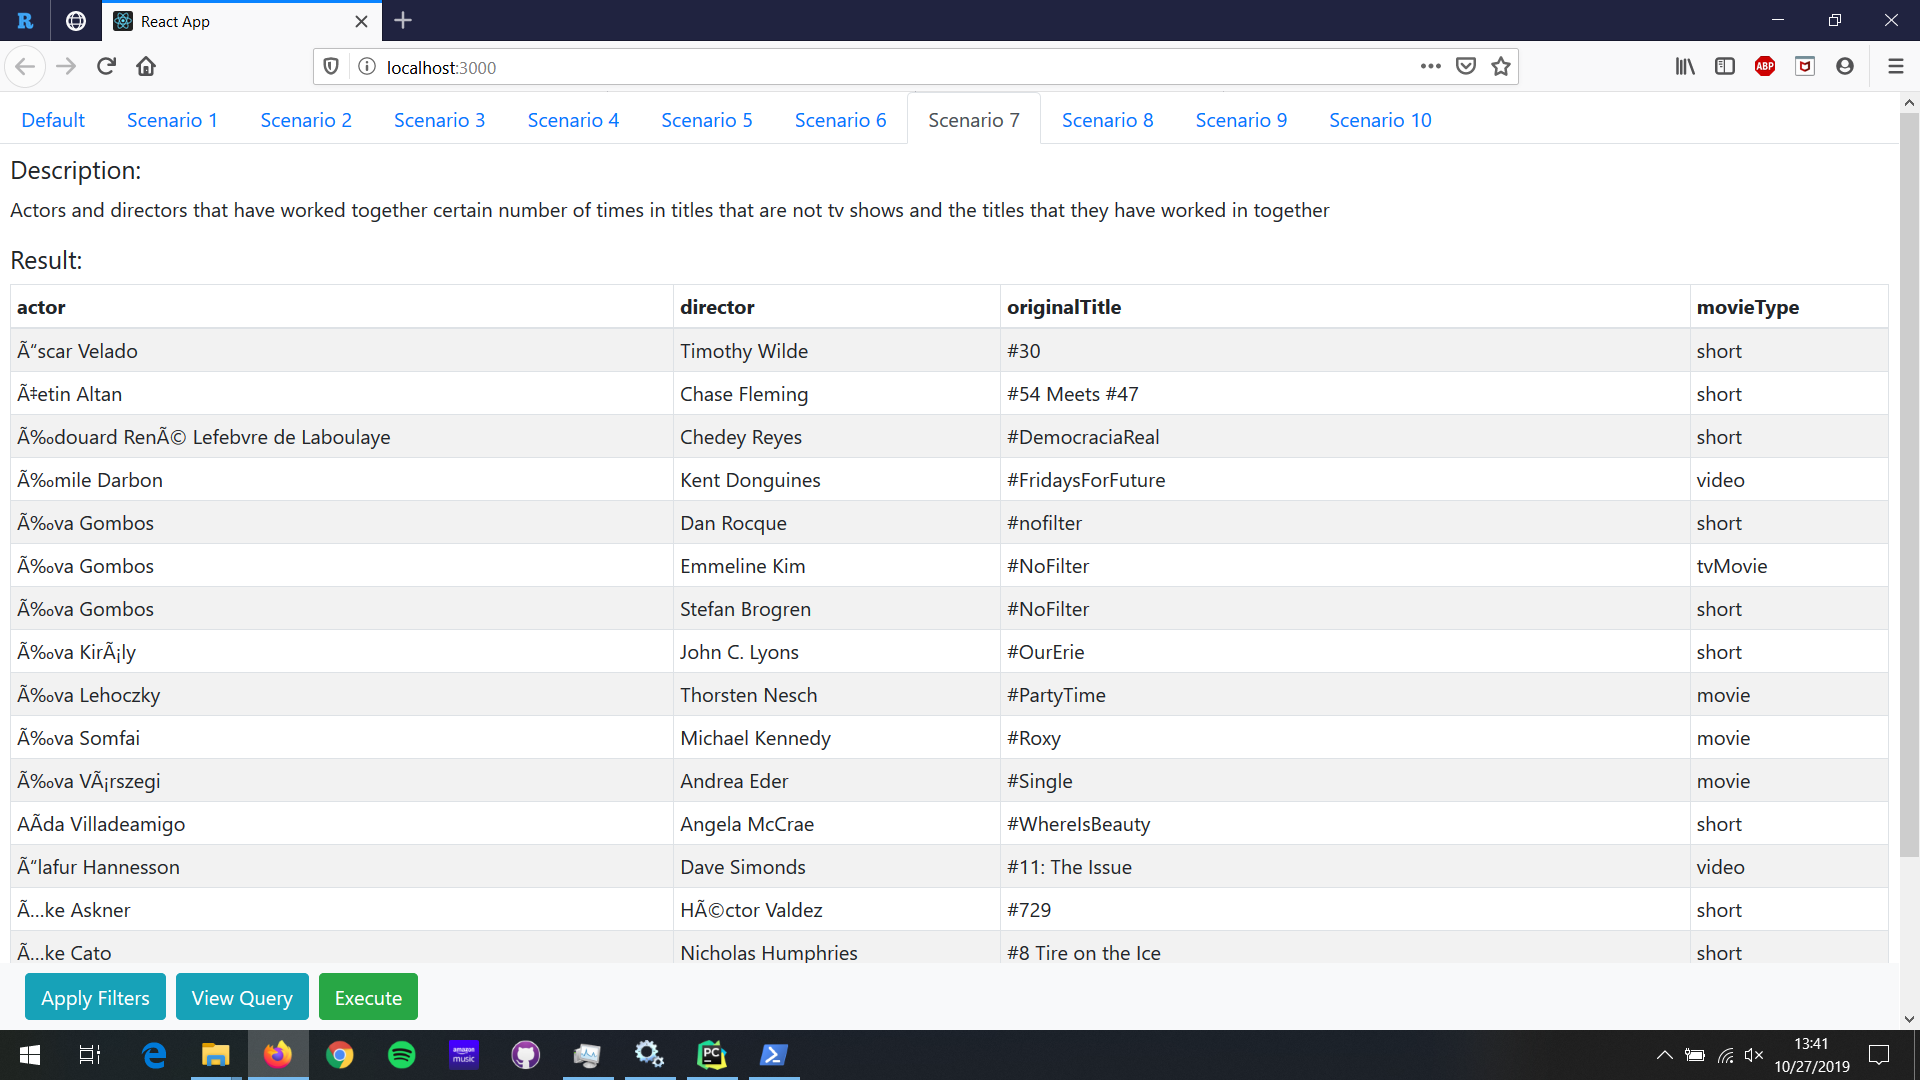
\includegraphics[width=8cm]{Screenshots/Scenario7.png}
		    \label{frontend}
                    \caption{Scenario 7 Result}
		    \centering
	        \end{figure}
		\item The highest rated episodes of shows that have spanned more than one year and have ended, by year sorted highest to lowest.
                \begin{lstlisting}
select top 100 e.originalTitle, e.startYear, t.averageRating
from tvEpisode e
inner join title t on e.originalTitle = t.originalTitle and e.primaryTitle = t.primaryTitle and e.startYear = t.startYear
inner join ( select s.originalTitle, s.primaryTitle, s.startYear, MAX(t.averageRating) as maxRating
from tvEpisode e
inner join title t on e.originalTitle = t.originalTitle and e.primaryTitle = t.primaryTitle and e.startYear = t.startYear
inner join tvSeries s on s.originalTitle = e.seriesOriginalTitle and s.primaryTitle = e.seriesPrimaryTitle and s.startYear = e.seriesStartYear
where s.endYear is not null and s.startYear <> s.endYear
group by s.originalTitle, s.primaryTitle, s.startYear ) r on r.originalTitle = e.seriesOriginalTitle and r.primaryTitle = e.seriesPrimaryTitle and r.startYear = e.seriesStartYear
where t.averageRating = r.maxRating;
                \end{lstlisting}
         	\begin{figure}[ht]
		    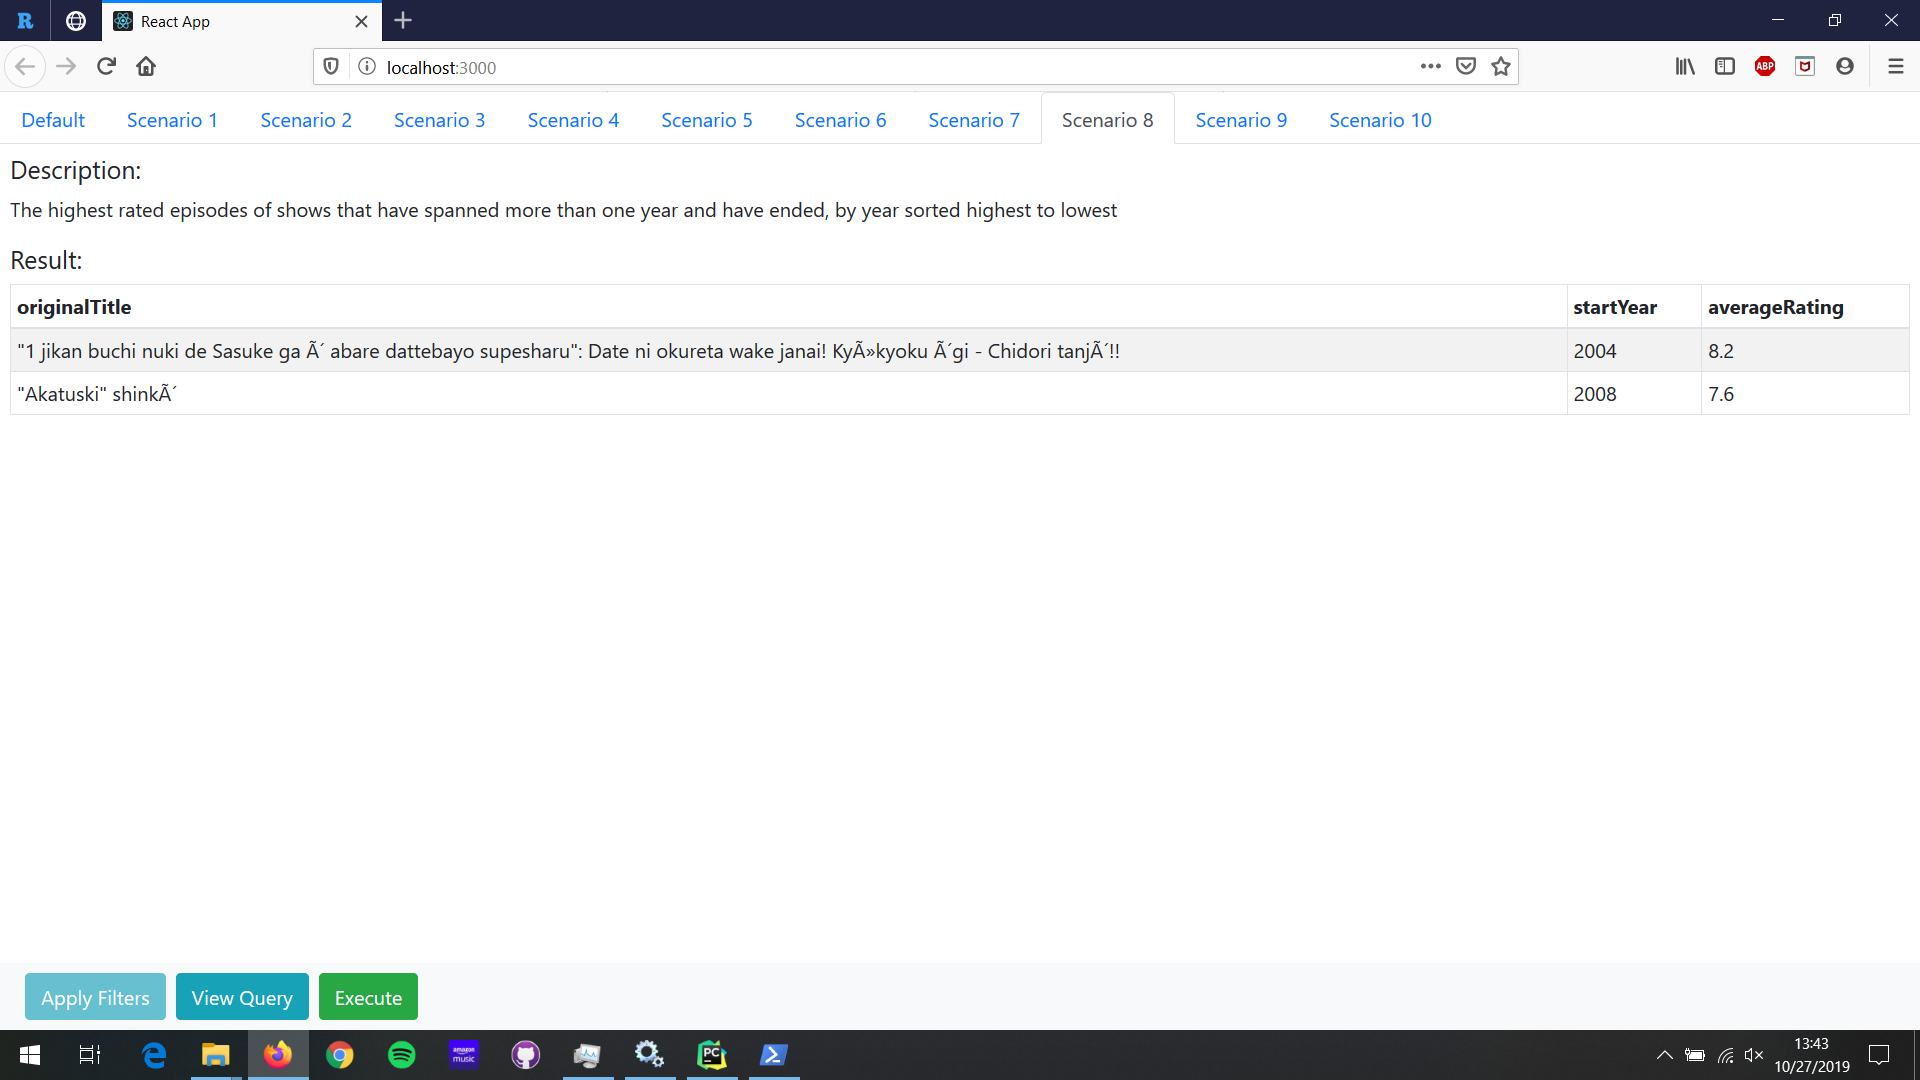
\includegraphics[width=8cm]{Screenshots/Scenario8.png}
		    \label{frontend}
                    \caption{Scenario 8 Result}
		    \centering
	        \end{figure}
		\item Writer, director that have worked together in atleast x different TV Shows
                \begin{lstlisting}
select top 100 w.primaryName as writer, d.primaryName as director
from writers w
inner join directors d on d.originalTitle = d.originalTitle and d.startYear = w.startYear
inner join tvSeries s on s.originalTitle = d.originalTitle and s.startYear = d.startYear
group by w.primaryName, w.birthYear, d.primaryName, d.birthYear
having COUNT(CONCAT(d.originalTitle, d.primaryTitle, d.startYear)) > 5;
                \end{lstlisting}
         	\begin{figure}[ht]
		    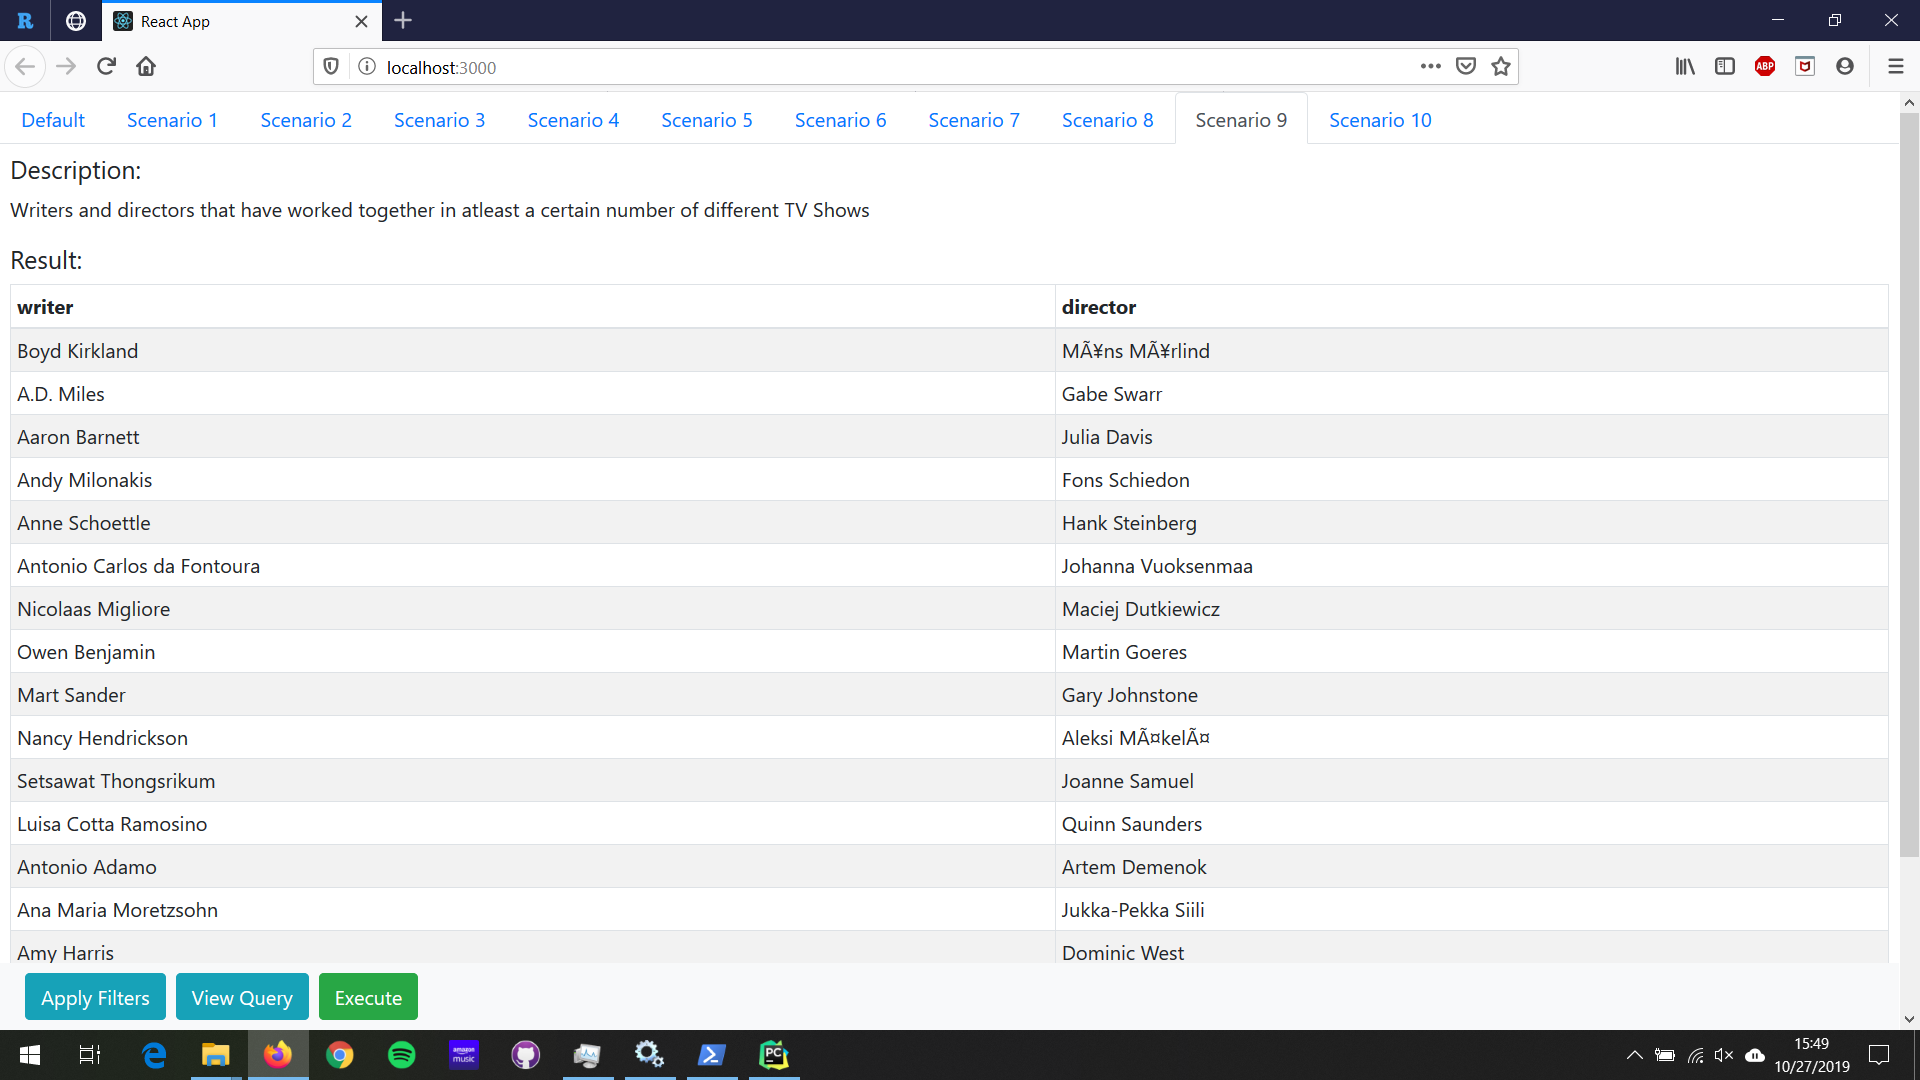
\includegraphics[width=8cm]{Screenshots/Scenario9.png}
		    \label{frontend}
                    \caption{Scenario 9 Result}
		    \centering
	        \end{figure}
		\item List the most popular TV shows between the years x and y that are still running.
                \begin{lstlisting}
select top 100 s.originalTitle, s.primaryTitle, s.startYear
from tvSeries s
inner join title t on s.originalTitle = t.originalTitle and s.primaryTitle = t.primaryTitle and s.startYear = t.startYear
inner join ( select t.startYear, MAX(t.averageRating) as maxRating
from title t
inner join tvSeries s on s.originalTitle = t.originalTitle and s.primaryTitle = t.primaryTitle and s.startYear = t.startYear
where s.endYear is not null and s.startYear between 2017 and 2019
group by t.startYear ) r on r.startYear = s.startYear
where t.averageRating = r.maxRating;'.format(startYear, endYear);
                \end{lstlisting}
                \textbf{Result:}
         	\begin{figure}[ht]
		    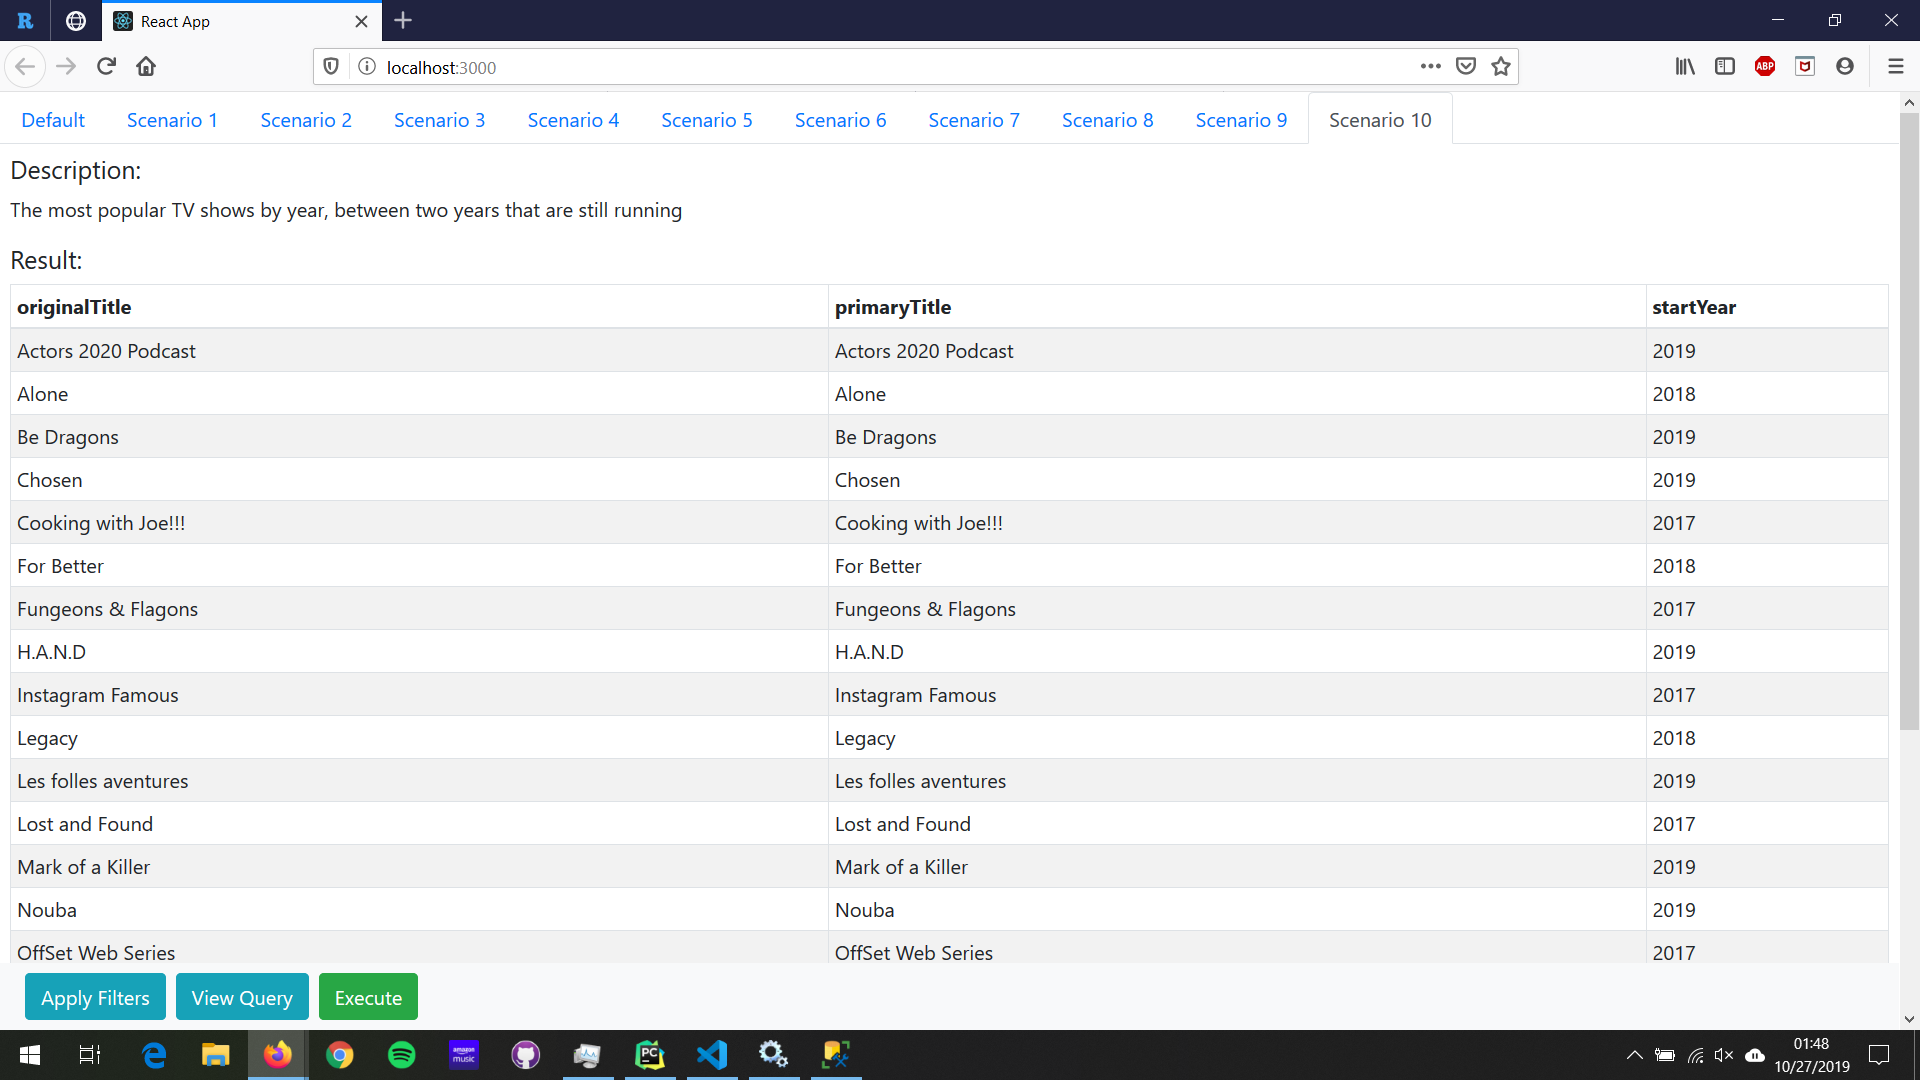
\includegraphics[width=8cm]{Screenshots/Scenario10.png}
                    \caption{Scenario 10 Result}
		    \label{frontend}
		    \centering
	        \end{figure}
	\end{enumerate}
	
	
\end{document}
